{
	\setbeamertemplate{footline}{} % Remove the footline for this slide only
	\begin{frame}
		\begin{figure}
			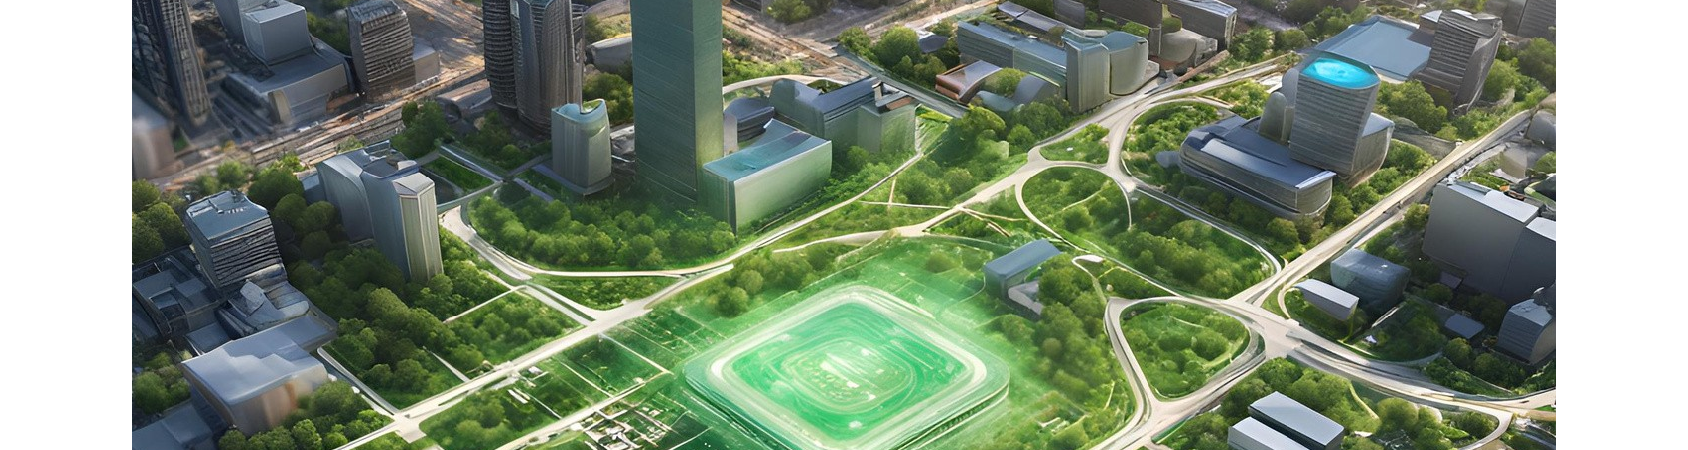
\includegraphics[width=\textwidth]{slides/figures/cover_image.pdf}
		\end{figure}
		\titlepage % This command creates the title page
		\vfill % This command will push your images to the bottom of the page
		
    \begin{figure}
	\centering % This centers the figure in the slide
	\begin{minipage}[b]{0.24\linewidth} % Adjust the width to accommodate four logos
		
\includegraphics[height=1.5em,keepaspectratio]{../figures/UHB_Logo_4c.pdf} % Existing logo 1
	\end{minipage}
	\hfill % This command inserts a space between the minipages
	\begin{minipage}[b]{0.24\linewidth} % Adjust the width for the second logo
		
\includegraphics[height=1.5em,keepaspectratio]{../figures/conahcyt.pdf} % Existing logo 2
	\end{minipage}
	\hfill % Space
\begin{minipage}[b]{0.24\linewidth} % New logo space
	
\includegraphics[height=2.5em,keepaspectratio]{../figures/NXP_Logo_RGB_Colour.png} % New NXP logo
\end{minipage}
	\hfill % Space
	\begin{minipage}[b]{0.24\linewidth} % Adjust the width for the third logo
		
\includegraphics[height=1.5em,keepaspectratio]{../figures/logo_item_ids.png} % Existing logo 3
	\end{minipage}

\end{figure}
		
		\addtocounter{framenumber}{-1} % this decrements the frame counter so the title page doesn't count
	\end{frame}
}
